\chapter{Contraction musculaire et motricité}\label{ch:b2:muscle-movement}

Une sprinteuse quitte les starting-blocks en exerçant sur la piste une
force de trois fois son poids, développée en un cinquième de seconde par
des muscles qui étaient relâchés l'instant d'avant. Rien dans la cellule
n'a raccourci pour cela~: les filaments intérieurs ont glissé les uns le
long des autres, tirés par des millions de mains moléculaires qui font
chacune un pas de dix nanomètres puis lâchent prise, dix fois par
seconde, au prix d'un ATP à chaque fois. Ce chapitre reprend la \omterm{def:b2:cell-differentiation:myogenesis}{fibre
musculaire} construite au \cref{ch:b2:cell-differentiation}
et la fait travailler~: le \omterm{prop:b2:muscle-movement:sliding}{glissement des filaments} et le moteur qui les
entraîne, l'interrupteur calcique qui met ce moteur en marche et
l'arrête, la commande venue du nerf, la mécanique de la force et de la
vitesse, et la manière dont le système nerveux gradue l'ensemble, de la
secousse au sprint.

\section{Les filaments glissants}

\begin{proposition}[Le mécanisme de glissement des filaments]\label{prop:b2:muscle-movement:sliding}
\index{glissement des filaments}\index{sarcomere@sarcomère!contraction}
Lorsqu'une \omterm{def:b2:cell-differentiation:myogenesis}{fibre musculaire} raccourcit, ses \omterm{def:b2:cell-differentiation:fibre}{sarcomères} raccourcissent
(\cref{ch:b2:cell-differentiation}), mais ni les filaments épais
de myosine ni les filaments fins d'actine ne changent de longueur~: les
filaments fins glissent vers l'intérieur le long des filaments épais, la
bande I et la zone H se rétrécissent, et les disques Z se rapprochent. Le
chevauchement des deux ensembles de filaments est le lieu où la force
est engendrée, et un \omterm{def:b2:cell-differentiation:fibre}{sarcomère} engendre une force proportionnelle à ce
chevauchement~: à partir d'une longueur étirée de \qty{3.6}{\micro m},
sans chevauchement ni force, la force croît linéairement à mesure que
les filaments se chevauchent davantage, atteint un plateau vers
\qty{2.2}{\micro m}, où chaque tête de myosine fait face à l'actine,
et diminue de nouveau en dessous de \qty{2.0}{\micro m}, lorsque les
filaments fins se heurtent et que les filaments épais butent contre les
disques Z. La longueur de repos d'un muscle dans le corps se situe sur le
plateau --- ce qui est le premier indice de la manière dont la force est
produite.
\end{proposition}
\begin{proof}[Faits expérimentaux]
A.~F.~Huxley et Niedergerke, et H.~E.~Huxley et Hanson (1954),
mesurèrent les bandes de fibres isolées et de \omterm{def:b2:cell-differentiation:fibre}{myofibrilles} isolées au
microscope interférentiel et à contraste de phase pendant leur
raccourcissement~: la bande A gardait sa longueur, la bande I
rétrécissait, donc les filaments glissent. Gordon,
Huxley et Julian (1966) maintinrent une fibre isolée à des longueurs
fixées au moyen d'un dispositif à rétroaction qui gardait constante la
longueur des \omterm{def:b2:cell-differentiation:fibre}{sarcomères} d'un segment, et trouvèrent que la force était
proportionnelle au chevauchement des filaments épais et fins mesuré en
microscopie électronique --- la courbe tension--longueur, avec son
plateau et ses deux branches linéaires, exactement comme le prédit la
géométrie des filaments.
\end{proof}

\begin{omfigure}
\begin{minipage}[b]{0.5\linewidth}\centering
\begin{tikzpicture}[every node/.style={font=\scriptsize}]
  \foreach \y/\lab/\ov in {2.4/{relâché, \qty{2.6}{\micro m}}/0.9, 1.2/{contracté, \qty{2.0}{\micro m}}/0.3} {
    \begin{scope}[yshift=\y cm]
      \draw[very thick, omThm] (0,-0.35) -- (0,0.35); \draw[very thick, omThm] (4.4-2*\ov+1.0,-0.35) -- (4.4-2*\ov+1.0,0.35);
      \pgfmathsetmacro{\len}{4.4-2*\ov+1.0}
      \foreach \dy in {-0.25,0.05,0.25} { \draw[thick, omDef] (0,\dy) -- (1.5,\dy); \draw[thick, omDef] (\len,\dy) -- (\len-1.5,\dy); }
      \draw[line width=3pt, omExo!80!black] (\len/2-1.1,-0.1) -- (\len/2+1.1,-0.1);
      \node[right] at (\len+0.15,0) {\lab};
    \end{scope}
  }
  \node[align=center] at (2.7,0.1) {les filaments gardent leur longueur~;\\le chevauchement croît quand\\les disques Z se rapprochent};
\end{tikzpicture}
\end{minipage}\hfill
\begin{minipage}[b]{0.48\linewidth}\centering
\begin{tikzpicture}
\begin{axis}[
  width=\linewidth, height=4.8cm,
  axis x line=bottom, axis y line=left,
  xmin=1.2, xmax=3.8, ymin=0, ymax=1.15,
  xlabel={longueur du sarcomère (\unit{\micro m})}, ylabel={force (valeur relative)},
  xlabel style={font=\scriptsize, at={(axis description cs:0.5,-0.17)}, anchor=north},
  ylabel style={font=\scriptsize},
  tick label style={font=\scriptsize}, xtick={1.3,2.0,2.2,3.6}, ytick={0,0.5,1},
  clip=false,
]
\addplot[very thick, omDef] coordinates {(1.3,0) (1.65,0.5) (2.0,1) (2.2,1) (3.6,0)};
\node[font=\scriptsize, anchor=south] at (axis cs:2.1,1.02) {plateau};
\node[font=\scriptsize, anchor=west, align=left] at (axis cs:2.95,0.75) {chevauchement\\décroissant};
\end{axis}
\end{tikzpicture}
\end{minipage}

{\small À gauche~: un \omterm{def:b2:cell-differentiation:fibre}{sarcomère} relâché et contracté --- les filaments
fins (en bleu) glissent le long des filaments épais (en gris) sans changer
de longueur. À droite~: la courbe tension--longueur~: la force est
proportionnelle au chevauchement, maximale sur le plateau où se trouve le
muscle au repos.}
\end{omfigure}

\begin{omfigure}
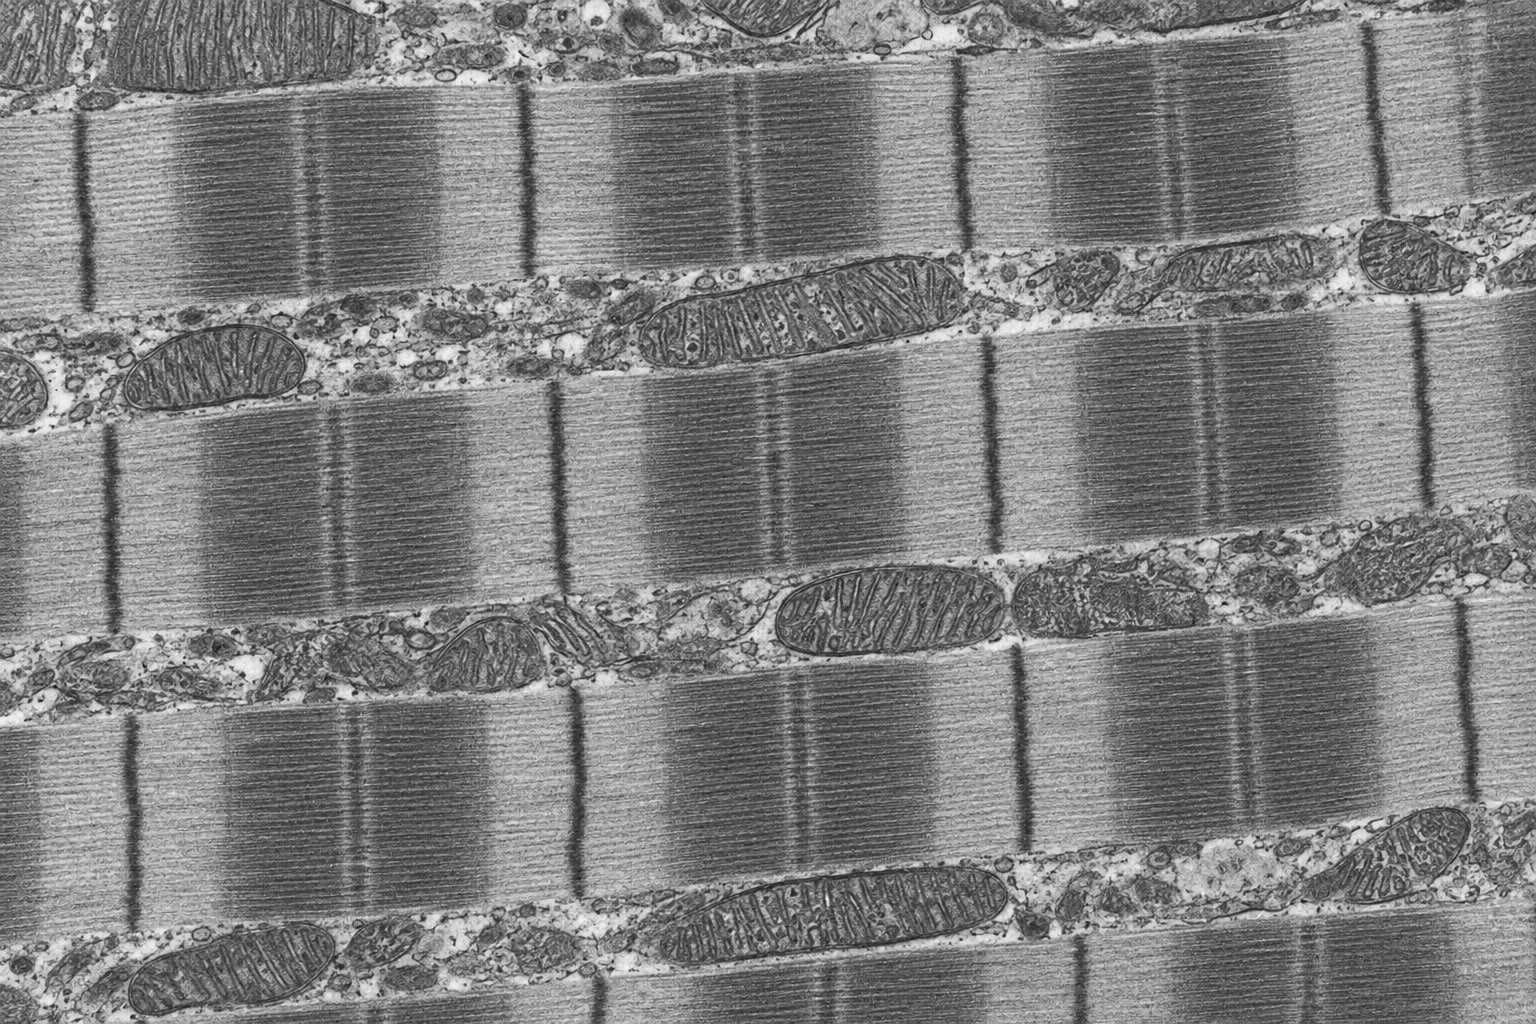
\includegraphics[width=0.6\linewidth]{images/book4/ai/b4-21-sarcomere-tem.jpg}

{\small Des \omterm{def:b2:cell-differentiation:fibre}{myofibrilles} au microscope électronique~: les bandes A de
filaments épais, les bandes I de filaments fins coupées en deux par les
stries Z, et les mitochondries situées entre les fibrilles, qui paient
le glissement.}
\end{omfigure}

\section{Le moteur}

\begin{proposition}[Le cycle des ponts d'union]\label{prop:b2:muscle-movement:crossbridge}
\index{cycle des ponts d'union}\index{myosine}\index{ATP!dans la contraction}
Chaque filament épais est hérissé de quelque trois cents \emph{têtes de
myosine}, et chaque tête est un moteur qui avance le long de l'actine au
cours d'un cycle en quatre étapes. (1) Lorsque l'ATP est fixé, la tête
est détachée de l'actine~; elle hydrolyse l'ATP en ADP et phosphate et
s'arme dans une conformation tendue, riche en énergie. (2) La tête armée
se fixe sur une sous-unité d'actine, formant un \emph{pont d'union}.
(3) Le phosphate est libéré et la tête revient brusquement à sa
conformation relâchée, tirant le filament fin d'environ \qty{10}{nm} vers
le centre du \omterm{def:b2:cell-differentiation:fibre}{sarcomère} --- le \emph{coup de rame}~; l'ADP s'en va. (4) Un
nouvel ATP se fixe et la tête lâche l'actine~; sans ATP, elle ne peut
pas lâcher prise, ce qui est la rigidité cadavérique. Le cycle dure
environ un vingtième de seconde~; une tête en passe la plus grande partie
détachée, si bien qu'à chaque instant seule une fraction des têtes tire,
et un filament qui glisse à vive allure n'est jamais lâché.
La force est la somme des tractions des têtes attachées~; le
raccourcissement est la somme de leurs pas, au plus un demi-micromètre
par \omterm{def:b2:cell-differentiation:fibre}{sarcomère} et par cycle~; et l'énergie est d'un ATP par pas et par
tête, environ \qty{50}{kJ/mol} --- \qty{8e-20}{J} par pas, dont la tête
convertit jusqu'à la moitié en travail.
\end{proposition}

\begin{omfigure}
\begin{tikzpicture}[every node/.style={font=\scriptsize}, >=stealth]
  \foreach \x/\lab/\ang/\att in {0/{1. ATP fixé~:\\tête détachée~; ATP\\hydrolysé, tête armée}/60/0, 3.6/{2. la tête armée\\se fixe sur l'actine~:\\pont d'union}/60/1, 7.2/{3. phosphate libéré~:\\coup de rame,\\filament tiré de \qty{10}{nm}}/20/1, 10.8/{4. l'ADP part, un nouvel\\ATP se fixe~: la tête\\lâche prise}/20/0} {
    \begin{scope}[xshift=\x cm]
      \draw[thick, omDef] (0,2.2) -- (2.8,2.2); \foreach \i in {0.2,0.6,...,2.6} \fill[omDef!50] (\i,2.2) circle (0.14);
      \draw[line width=3pt, omExo!80!black] (0,0.4) -- (2.8,0.4);
      \draw[very thick, omThm] (1.4,0.4) -- (1.4,1.0);
      \ifnum\att=1 \draw[very thick, omThm] (1.4,1.0) -- ++(\ang:1.15); \fill[omThm] (1.4,1.0) ++(\ang:1.15) circle (0.16); \else \draw[very thick, omThm] (1.4,1.0) -- ++(\ang:1.0); \fill[omThm] (1.4,1.0) ++(\ang:1.0) circle (0.16); \fi
      \node[below, align=center] at (1.4,0.15) {\lab};
    \end{scope}
  }
  \draw[->, thick, omDef] (7.9,2.55) -- (8.9,2.55); \node[omDef, above] at (8.4,2.6) {le filament fin avance};
\end{tikzpicture}

{\small Le \omterm{prop:b2:muscle-movement:crossbridge}{cycle des ponts d'union}. Une tête de myosine armée (en rouge)
se fixe sur l'actine (en bleu), libère le phosphate et tire le filament
fin par son coup de rame, puis fixe un nouvel ATP et lâche prise.}
\end{omfigure}

\begin{theorem}[Force, vitesse et puissance d'un muscle]\label{thm:b2:muscle-movement:hill}
\index{courbe force--vitesse}\index{puissance musculaire}
La force d'un muscle diminue lorsqu'il raccourcit plus vite, car plus
les filaments glissent vite, moins il y a de têtes attachées à chaque
instant, et plus nombreuses sont celles qui sont entraînées au-delà de
leur coup de rame avant de lâcher prise. La relation de Hill la décrit~:
\[
(F + a)(v + b) = (F_0 + a)\,b,
\]
où $F_0$ est la force isométrique (à $v = 0$), $v_{\max} =
F_0 b/a$ la vitesse à charge nulle, et $a$, $b$ des constantes ($a \approx
F_0/4$). La puissance $Fv$ est nulle aux deux extrémités et maximale
vers un tiers de $v_{\max}$ et un tiers de $F_0$ --- ce qui explique
qu'un cycliste change de vitesse et que la foulée d'un sprinteur ait une
cadence préférée. Un muscle humain développe environ \qty{30}{N} par
centimètre carré de section, raccourcit jusqu'à dix longueurs par
seconde, et fournit au mieux quelque \qty{100}{W} par kilogramme.
\end{theorem}
\begin{proof}
La courbe de Hill est empirique (1938), mesurée sur un muscle de
grenouille isolé comme la vitesse de raccourcissement en fonction de la
charge soulevée~; l'hyperbole convient parce que la fraction de têtes
attachées diminue avec la vitesse de glissement et que la force de chaque
tête attachée diminue à mesure qu'elle est entraînée au long de son coup
de rame. Puissance~: avec $F = (F_0 + a)b/(v + b) - a$, $Fv$ est nulle en
$v = 0$ et en $v_{\max}$~; la dérivation donne le maximum en
$v = b(\sqrt{(F_0 + a)/a} - 1)$, soit, pour $a = F_0/4$, $v =
1.24\,b = 0.31\,v_{\max}$, où $F = 0.31\,F_0$.
\end{proof}

\begin{omfigure}
\begin{tikzpicture}
\begin{axis}[
  width=0.7\linewidth, height=5.4cm,
  axis x line=bottom, axis y line=left,
  xmin=0, xmax=1.05, ymin=0, ymax=1.1,
  xlabel={vitesse de raccourcissement $v/v_{\max}$}, ylabel={force $F/F_0$, puissance (valeur relative)},
  xlabel style={font=\small, at={(axis description cs:0.5,-0.13)}, anchor=north},
  ylabel style={font=\small},
  tick label style={font=\small}, xtick={0,0.31,1}, xticklabels={0,0.31,1}, ytick={0,0.31,1}, yticklabels={0,0.31,1},
  legend style={font=\scriptsize, at={(0.97,0.95)}, anchor=north east, draw=none},
  clip=false,
]
\addplot[very thick, omDef, domain=0:1, samples=100] {(1.25*0.25)/(x+0.25) - 0.25};
\addlegendentry{force}
\addplot[very thick, omThm, domain=0:1, samples=100] {10.4*x*((1.25*0.25)/(x+0.25) - 0.25)};
\addlegendentry{puissance (mise à l'échelle)}
\draw[dashed, gray] (axis cs:0.31,0) -- (axis cs:0.31,1.0);
\end{axis}
\end{tikzpicture}

{\small La \omterm{thm:b2:muscle-movement:hill}{courbe force--vitesse} de Hill ($a = F_0/4$) et la puissance qui
en découle~: la force diminue lorsque le muscle raccourcit plus vite, et
la puissance culmine vers un tiers de la vitesse maximale et un tiers de
la force isométrique.}
\end{omfigure}

\section{L'interrupteur~: le calcium}

\begin{proposition}[Le couplage excitation--contraction]\label{prop:b2:muscle-movement:coupling}
\index{couplage excitation--contraction}\index{troponine}\index{tropomyosine}\index{reticulum sarcoplasmique@réticulum sarcoplasmique}
Au repos, les têtes de myosine ne peuvent pas atteindre l'actine~: les
sites de fixation du filament fin sont couverts par la
\emph{tropomyosine}, un bâtonnet couché dans le sillon de l'hélice
d'actine, maintenu en place par la \emph{troponine}.
L'interrupteur est le calcium. Un \omterm{prop:b2:neurons-synapses:ap}{potentiel d'action} sur la membrane de
la fibre descend le long des \omterm{def:b2:cell-differentiation:fibre}{tubules T} vers l'intérieur et, aux jonctions
où un \omterm{def:b2:cell-differentiation:fibre}{tubule T} rencontre le \omterm{def:b2:cell-differentiation:fibre}{réticulum sarcoplasmique}, ouvre les canaux de
libération du calcium du réticulum~; le calcium inonde les \omterm{def:b2:cell-differentiation:fibre}{myofibrilles},
passant de \qty{0.1}{} à \qty{10}{\micro mol/L} en une milliseconde, se
fixe sur la troponine, et la troponine écarte la tropomyosine des sites
de fixation~: les têtes s'attachent, et la fibre se contracte tant que le
calcium demeure. Des pompes du réticulum, consommant de l'ATP, reprennent
le calcium en quelques dizaines de millisecondes~; la tropomyosine
recouvre les sites et la fibre se relâche. Le relâchement est donc aussi
actif que la contraction, et un muscle privé d'ATP ne peut ni libérer ses
têtes ni pomper son calcium --- c'est la rigidité cadavérique. Le \omterm{def:b2:heart:anatomy}{cœur}
utilise le même interrupteur, mais avec du calcium venu de l'extérieur
par les propres canaux de la membrane pour déclencher la libération,
ce qui explique que le \omterm{def:b2:heart:anatomy}{cœur}, et non le muscle squelettique, soit sensible
au calcium du \omterm{def:b2:blood-circulation:blood}{sang}.
\end{proposition}

\begin{omfigure}
\begin{tikzpicture}[every node/.style={font=\scriptsize}, >=stealth]
  \node[draw, rounded corners, fill=omDef!15, align=center] (nerve) at (0,0) {influx du\\nerf moteur};
  \node[draw, rounded corners, fill=omDef!15, align=center] (nmj) at (3.0,0) {jonction\\neuromusculaire~:\\acétylcholine};
  \node[draw, rounded corners, fill=omDef!15, align=center] (ap) at (6.2,0) {potentiel d'action\\musculaire, le long\\des tubules T};
  \node[draw, rounded corners, fill=omThm!15, align=center] (ca) at (9.4,0) {Ca$^{2+}$ libéré\\par le réticulum\\sarcoplasmique};
  \node[draw, rounded corners, fill=omProp!20, align=center] (tn) at (12.6,0) {la troponine fixe Ca$^{2+}$,\\la tropomyosine se déplace,\\les têtes s'attachent};
  \node[draw, rounded corners, fill=omExo!25, align=center] (off) at (9.4,-2.2) {les pompes reprennent Ca$^{2+}$ (ATP)~;\\la tropomyosine recouvre l'actine~:\\relâchement};
  \draw[->, thick] (nerve) -- (nmj); \draw[->, thick] (nmj) -- (ap); \draw[->, thick] (ap) -- (ca); \draw[->, thick] (ca) -- (tn);
  \draw[->, thick] (ca) -- (off);
  \node[below, gray] at (1.5,-0.7) {\qty{0.6}{ms}}; \node[below, gray] at (4.6,-0.7) {\qty{1}{ms}}; \node[below, gray] at (7.8,-0.7) {\qty{1}{ms}};
\end{tikzpicture}

{\small De l'influx nerveux à la force~: la jonction, le \omterm{prop:b2:neurons-synapses:ap}{potentiel d'action}
propre de la fibre, la libération du calcium et le dégagement des sites
de l'actine --- puis les pompes qui y mettent fin.}
\end{omfigure}

\section{Commande et gradation}

\begin{definition}[L'unité motrice]\label{def:b2:muscle-movement:motorunit}
\index{unite motrice@unité motrice}\index{secousse musculaire}\index{tetanos@tétanos}\index{recrutement}
Un \emph{motoneurone} de la moelle épinière envoie son \omterm{def:b2:neurons-synapses:neuron}{axone} vers un
muscle et se ramifie pour innerver de quelques fibres à un millier,
dispersées dans le muscle~; le \omterm{def:b2:neurons-synapses:neuron}{neurone} et ses fibres forment une
\emph{unité motrice}, la plus petite quantité de force que le système
nerveux puisse commander. Chaque influx du \omterm{def:b2:neurons-synapses:neuron}{neurone} fait décharger une
fois chaque fibre de l'unité, qui produit une \emph{secousse}~: une
force qui monte en quelque \qty{30}{ms} et décroît en \qty{100}{ms},
parce que l'impulsion calcique est brève. Des influx en succession
rapide font se sommer les secousses, puisque le calcium de l'une n'a pas
été repompé lorsque la suivante arrive~; vers 30 à 50 influx par seconde,
la force fusionne en un \emph{tétanos} lisse, trois à cinq fois la
secousse. Le système nerveux gradue la force d'un muscle de deux
manières~: par la \emph{fréquence} de décharge de chaque unité, et par le
\emph{nombre} d'unités qu'il recrute --- les petites unités lentes et
résistantes à la fatigue d'abord (le \emph{principe de taille}), les
grandes unités rapides en dernier, pour les efforts les plus grands
seulement. Un muscle en usage ordinaire n'est donc jamais pleinement
activé~: une fraction de ses unités décharge, à tour de rôle, et les
autres se reposent.
\end{definition}

\begin{omfigure}
\begin{tikzpicture}
\begin{axis}[
  width=0.82\linewidth, height=5.4cm,
  axis x line=bottom, axis y line=left,
  xmin=0, xmax=1.0, ymin=0, ymax=4.2,
  xlabel={temps (s)}, ylabel={force (secousse $=$ 1)},
  xlabel style={font=\small, at={(axis description cs:0.5,-0.13)}, anchor=north},
  ylabel style={font=\small},
  tick label style={font=\small}, xtick={0,0.2,0.4,0.6,0.8,1}, ytick={0,1,2,3,4},
  clip=false,
]
% single twitch
\addplot[very thick, omDef, domain=0:0.2, samples=60] {(x<0.02)*0 + (x>=0.02)*4.5*(x-0.02)*exp(-(x-0.02)/0.03)*4.1};
% summation at 10 Hz
\addplot[very thick, omProp, domain=0.25:0.62, samples=200] {(x>=0.25)*4.5*4.1*(x-0.25)*exp(-(x-0.25)/0.03) + (x>=0.33)*4.5*4.1*(x-0.33)*exp(-(x-0.33)/0.03) + (x>=0.41)*4.5*4.1*(x-0.41)*exp(-(x-0.41)/0.03) + (x>=0.49)*4.5*4.1*(x-0.49)*exp(-(x-0.49)/0.03)};
% tetanus at 50 Hz
\addplot[very thick, omThm, domain=0.66:0.98, samples=100] {3.8*(1-exp(-(x-0.66)/0.06))};
\node[font=\scriptsize, anchor=west] at (axis cs:0.09,0.7) {un influx~: secousse};
\node[font=\scriptsize, anchor=south] at (axis cs:0.44,2.2) {\qty{12}{Hz}~: sommation};
\node[font=\scriptsize, anchor=south] at (axis cs:0.82,3.85) {\qty{50}{Hz}~: tétanos fusionné};
\end{axis}
\end{tikzpicture}

{\small Graduer la force par la fréquence. Un influx isolé donne une
secousse~; des influx à une douzaine par seconde se somment en une force
ondulante~; à cinquante par seconde, la force fusionne en un \omterm{def:b2:muscle-movement:motorunit}{tétanos} de
plusieurs fois la secousse.}
\end{omfigure}

\begin{proposition}[Les réflexes et la moelle épinière]\label{prop:b2:muscle-movement:reflex}
\index{arc reflexe@arc réflexe}\index{fuseau neuromusculaire}\index{reflexe myotatique@réflexe myotatique}\index{inhibition reciproque@inhibition réciproque}
Le motoneurone est la \emph{voie finale commune}~: toute commande, venue
du cortex ou d'un réflexe, aboutit à lui. Le circuit le plus simple
est le \emph{\omterm{prop:b2:muscle-movement:reflex}{réflexe myotatique}} du \cref{ch:b2:neurons-synapses}~:
des terminaisons sensitives enroulées autour de fibres spéciales situées
dans le muscle, les \emph{fuseaux neuromusculaires}, déchargent lorsque
le muscle est étiré, excitent par une seule \omterm{def:b2:neurons-synapses:synapse}{synapse} les motoneurones du
même muscle et inhibent ceux de l'antagoniste par un interneurone
(l'\emph{\omterm{prop:b2:muscle-movement:reflex}{inhibition réciproque}}), si bien que le muscle résiste à
l'étirement --- la base de la posture, puisque chaque oscillation étire
un muscle. Un second récepteur, l'organe tendineux, décharge lorsque la
force du muscle est élevée et inhibe les motoneurones du muscle
lui-même~: une soupape de sécurité. Le retrait devant un stimulus
douloureux est un réflexe à plusieurs \omterm{def:b2:neurons-synapses:synapse}{synapses} qui fléchit le membre et,
de l'autre côté, étend le membre opposé pour éviter la chute. Et le
cerveau ne commande pas des muscles mais des mouvements~: le cortex
envoie un plan, le cervelet le corrige d'après ce que rapportent les
fuseaux, les noyaux gris centraux le libèrent, et les circuits de la
moelle épinière, capables d'entretenir seuls un rythme de marche,
l'exécutent --- le sujet du volume de troisième année.
\end{proposition}

\begin{omfigure}
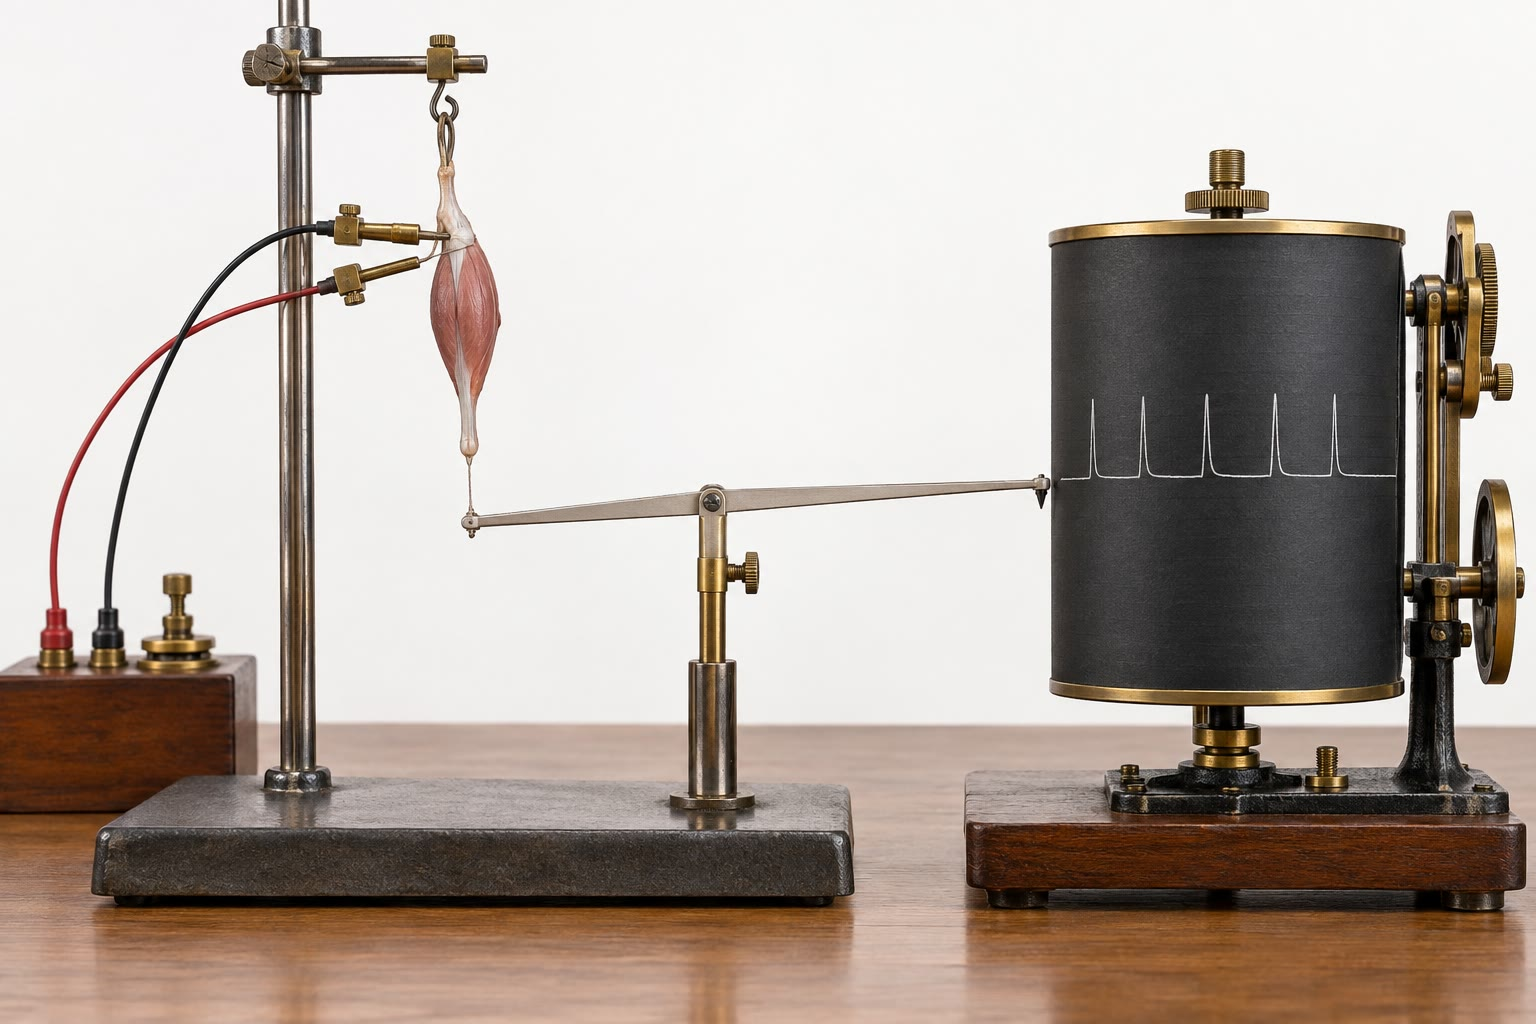
\includegraphics[width=0.44\linewidth]{images/book4/ai/b4-21-frog-muscle-prep.jpg}\hspace{0.04\linewidth}
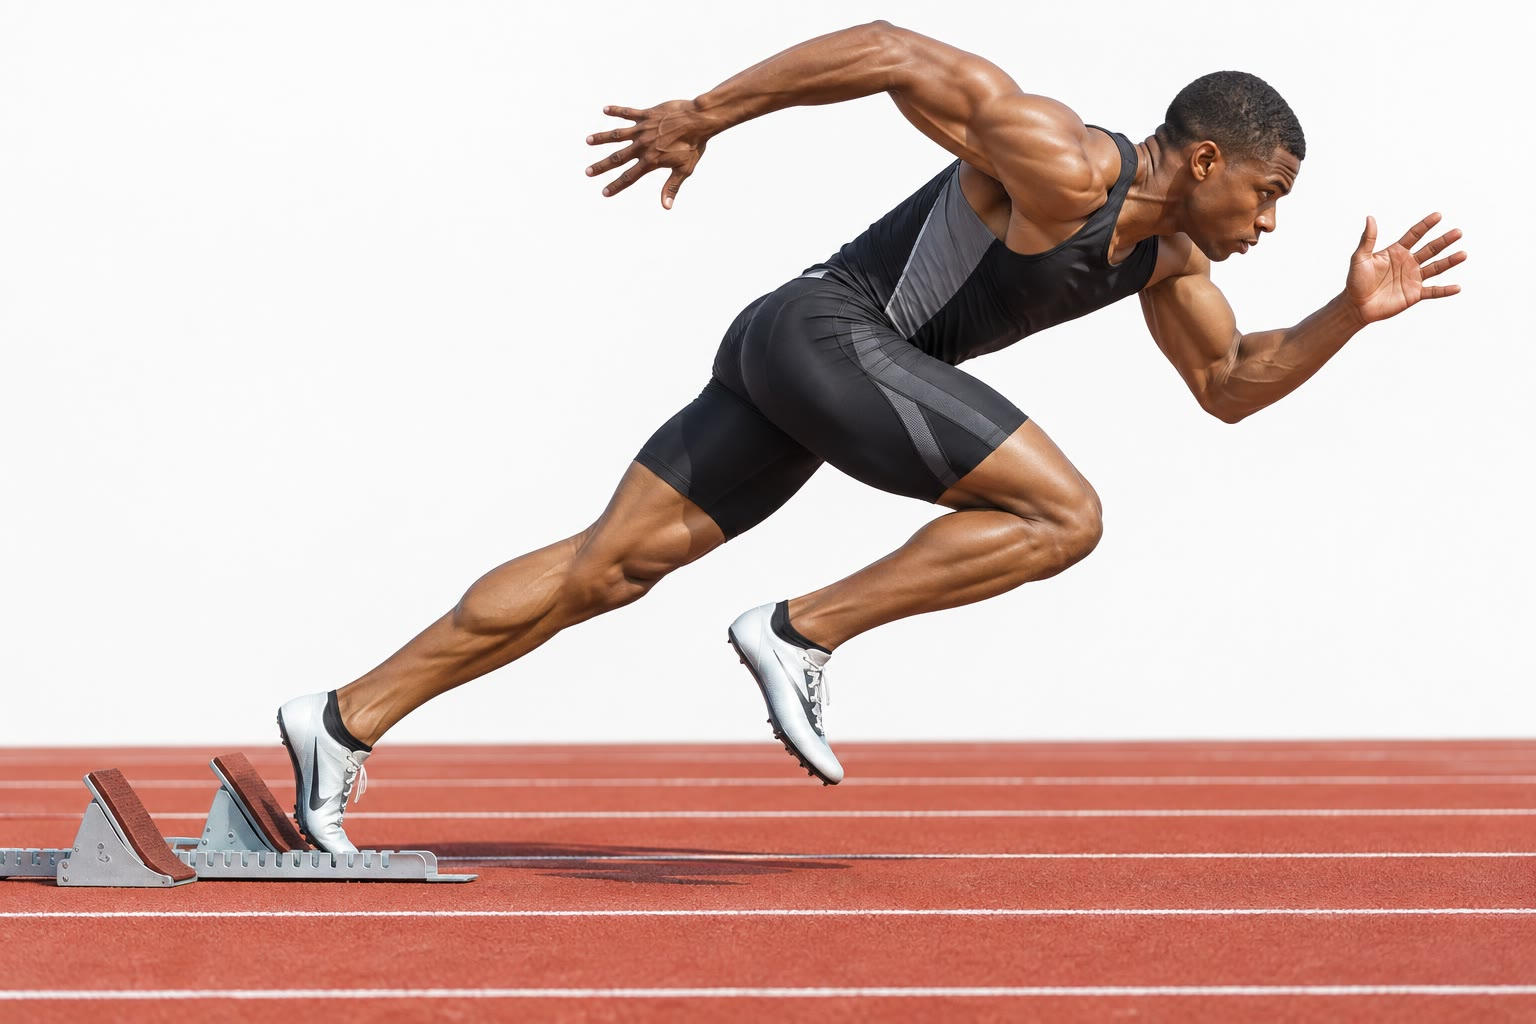
\includegraphics[width=0.44\linewidth]{images/book4/ai/b4-21-sprinter.jpg}

{\small À gauche~: la préparation classique --- un muscle de grenouille,
son nerf, des électrodes de stimulation et un levier inscrivant sur un
cylindre enfumé --- sur laquelle secousse, sommation et \omterm{def:b2:muscle-movement:motorunit}{tétanos} furent
enregistrés pour la première fois. À droite~: la même physiologie en
plein effort.}
\end{omfigure}

\section{Carburant et fatigue}

\begin{proposition}[Payer le travail]\label{prop:b2:muscle-movement:energy}
\index{phosphocreatine@phosphocréatine}\index{fatigue musculaire}\index{dette d'oxygene@dette d'oxygène}
Une fibre contient de l'ATP pour une ou deux secondes d'effort maximal.
La première réserve est la \emph{phosphocréatine}, qui rephosphoryle
l'ADP en quelques millisecondes et dure une dizaine de secondes --- le
carburant du sprinteur. La deuxième est la \emph{glycolyse} du glycogène
de la fibre, sans oxygène, qui rend deux ATP par glucose et du lactate~:
rapide, suffisante pour une minute ou deux, et autolimitée par
l'accumulation d'acide et de phosphate. La troisième est le métabolisme
\emph{oxydatif} du glucose et des acides gras dans les mitochondries,
trente ATP par glucose, limité seulement par l'oxygène qu'apporte le \omterm{def:b2:blood-circulation:blood}{sang}
(\cref{ch:b2:blood-pressure})~: le marathon. Les fibres rapides
glycolytiques s'appuient sur les deux premières et se fatiguent en une
minute~; les fibres lentes oxydatives, rouges de myoglobine et remplies de
mitochondries, fonctionnent pendant des heures.
La \emph{fatigue} d'un effort bref n'est pas l'épuisement de l'ATP ---
qui laisserait le muscle en rigidité --- mais l'accumulation de phosphate
et de protons, qui affaiblissent les ponts d'union et la libération du
calcium~; dans un effort long, c'est l'épuisement du glycogène et,
finalement, de la volonté. Après l'effort, le muscle rembourse sa
\emph{\omterm{prop:b2:muscle-movement:energy}{dette d'oxygène}}~: il restaure la phosphocréatine, reconvertit le
lactate (dans le foie) et reconstitue ses réserves, en respirant fort
pendant des minutes après s'être immobilisé.
\end{proposition}

\begin{example}[Un cent mètres]\label{ex:b2:muscle-movement:sprint}
Dix secondes d'effort maximal par \qty{20}{kg} de muscles des jambes à
\qty{100}{W/kg} représentent \qty{2}{kW} de puissance mécanique et, avec
un rendement de \qty{25}{\%}, \qty{8}{kW} de renouvellement de l'ATP ---
quelque \qty{160}{mmol} d'ATP par seconde, soit \qty{800}{g} d'ATP sur la course.
Le muscle en contient une cinquantaine de grammes~; la phosphocréatine fournit les
cinq premières secondes, la glycolyse le reste, et la sprinteuse termine
avec un lactate sanguin de \qty{15}{mmol/L} et une dette qu'elle
rembourse au cours du quart d'heure suivant. Une marathonienne à
\qty{300}{W} pendant deux heures produit \qty{2}{MJ} de travail et brûle
\qty{8}{MJ} de carburant --- un kilogramme de glycogène et de graisse ---
avec un apport d'oxygène de \qty{4}{L/min} tout du long, et le mur
qu'elle heurte au trentième kilomètre est le fond de ses réserves de
glycogène.
\end{example}
\section{Exercices}

\begin{exercise}[$\star$]\label{exo:b2:muscle-movement:1}
Énoncer le mécanisme de \omterm{prop:b2:muscle-movement:sliding}{glissement des filaments} et dire quelles bandes
du \omterm{def:b2:cell-differentiation:fibre}{sarcomère} changent lors de la contraction et lesquelles ne changent
pas.
\end{exercise}

\begin{exercise}[$\star$]\label{exo:b2:muscle-movement:2}
Donner les quatre étapes du \omterm{prop:b2:muscle-movement:crossbridge}{cycle des ponts d'union} et le rôle de l'ATP
dans chacune. Pourquoi un muscle privé d'ATP devient-il rigide~?
\end{exercise}

\begin{exercise}[$\star$]\label{exo:b2:muscle-movement:3}
Énumérer les événements qui mènent d'un influx du nerf moteur à
l'attachement des têtes de myosine, avec la durée de chacun.
\end{exercise}

\begin{exercise}[$\star$]\label{exo:b2:muscle-movement:4}
Définir \omterm{def:b2:muscle-movement:motorunit}{unité motrice}, secousse et \omterm{def:b2:muscle-movement:motorunit}{tétanos}, et donner les deux manières
dont le système nerveux gradue la force.
\end{exercise}

\begin{exercise}[$\star\star$]\label{exo:b2:muscle-movement:5}
Un \omterm{def:b2:cell-differentiation:fibre}{sarcomère} de \qty{2.4}{\micro m} raccourcit à \qty{2.0}{\micro m} en
\qty{50}{ms}. Calculer la vitesse de \omterm{prop:b2:muscle-movement:sliding}{glissement des filaments} fins par
rapport aux filaments épais et, avec un pas de \qty{10}{nm}, le nombre
de cycles que chaque tête attachée doit effectuer par seconde.
\end{exercise}

\begin{exercise}[$\star\star$]\label{exo:b2:muscle-movement:6}
Une fibre de \qty{10}{cm} compte \num{40000} \omterm{def:b2:cell-differentiation:fibre}{sarcomères} en série et
raccourcit de \qty{20}{\%} en \qty{0.1}{s}. Calculer sa vitesse de
raccourcissement en longueurs par seconde et en mètres par seconde, et
la vitesse de chaque \omterm{def:b2:cell-differentiation:fibre}{sarcomère}.
\end{exercise}

\begin{exercise}[$\star\star$]\label{exo:b2:muscle-movement:7}
Avec la relation de Hill, $a = F_0/4$ et $v_{\max} = 10$ longueurs par
seconde, calculer la force (en fraction de $F_0$) à 1, 3 et 6
longueurs par seconde, et la puissance dans chaque cas. Où la puissance
est-elle maximale~?
\end{exercise}

\begin{exercise}[$\star\star$]\label{exo:b2:muscle-movement:8}
Un quadriceps de \qty{80}{cm^2} de section à \qty{30}{N/cm^2}~:
calculer sa force isométrique maximale. Il s'insère à \qty{5}{cm} de
l'articulation du genou sur un levier dont le pied est à \qty{45}{cm} de
l'articulation~: quelle force le pied peut-il exercer~?
\end{exercise}

\begin{exercise}[$\star\star$]\label{exo:b2:muscle-movement:9}
L'impulsion calcique d'une secousse dure \qty{30}{ms}. Expliquer pourquoi
des influx à \qty{10}{Hz} donnent une force ondulante, à \qty{50}{Hz} un
\omterm{def:b2:muscle-movement:motorunit}{tétanos} lisse, et pourquoi la force tétanique dépasse la secousse.
\end{exercise}

\begin{exercise}[$\star\star\star$]\label{exo:b2:muscle-movement:10}
Les \qty{20}{kg} de muscles des jambes d'une sprinteuse fournissent
\qty{2}{kW} pendant \qty{10}{s} avec un rendement de \qty{25}{\%}.
Calculer l'ATP utilisé (\qty{50}{kJ/mol}), la phosphocréatine nécessaire
pour couvrir les \qty{5}{s} premières, et le glucose fermenté pour
couvrir le reste (2 ATP par glucose). Quelle concentration de lactate
cela produit-il dans \qty{40}{L} d'eau corporelle~?
\end{exercise}

\begin{exercise}[$\star\star\star$]\label{exo:b2:muscle-movement:11}
Prévoir l'effet sur la contraction~: d'un médicament qui bloque le canal
de libération du calcium du réticulum~; d'un médicament qui bloque sa
pompe~; d'une \omterm{def:b2:genome-diversification:mutation}{mutation} qui rend la troponine insensible au calcium~; de
la suppression du calcium sanguin, pour le muscle squelettique et pour le
\omterm{def:b2:heart:anatomy}{cœur}.
\end{exercise}

\begin{exercise}[$\star\star\star$]\label{exo:b2:muscle-movement:12}
«~Un muscle est une machine qui convertit l'énergie chimique en force
avec le rendement d'un bon moteur et le contrôle d'un ordinateur.~»
Discuter le rendement (un quart à une moitié), ce qui le limite, et ce
que les deux manières dont le système nerveux gradue la force apportent
qu'un simple interrupteur n'apporterait pas.
\end{exercise}

\section{Problème~: la physiologie d'un saut}

\begin{problem}[{Problème du week-end --- un saut sans élan analysé du
sarcomère à l'impulsion~: le glissement, les ponts d'union,
l'interrupteur calcique, la limite force--vitesse, les unités motrices et
le carburant, jusqu'au nombre de coups de rame des ponts d'union, à la
force disponible à la vitesse d'impulsion et à l'ATP que coûte le saut}]
\label{pb:b2:muscle-movement:1}
Une personne de \qty{70}{kg} saute à \qty{40}{cm} à la verticale,
élevant le centre de masse du corps de \qty{0.4}{m} pendant une poussée
de \qty{0.3}{s}. Les extenseurs des jambes (\qty{20}{kg} de muscle) ont
une section totale de \qty{500}{cm^2} à \qty{30}{N/cm^2}~; leurs fibres
mesurent \qty{12}{cm} (\num{48000} \omterm{def:b2:cell-differentiation:fibre}{sarcomères}) et raccourcissent de
\qty{4}{cm} pendant la poussée~; les articulations multiplient le
raccourcissement du muscle par \num{10} au niveau du pied et divisent sa
force par le même facteur. $v_{\max} = 8$ longueurs par seconde, $a = F_0/4$. Chaque
filament épais porte \num{300} têtes de myosine~; il y a $6\times
10^{10}$ filaments épais par centimètre carré de muscle~; un coup de rame
mesure \qty{10}{nm} et coûte un ATP (\qty{8e-20}{J}, \qty{50}{kJ/mol})~;
rendement \qty{40}{\%}. Le muscle contient \qty{5}{mmol/kg} d'ATP et
\qty{20}{mmol/kg} de phosphocréatine. Les fibres ont un diamètre de \qty{60}{\micro
m}. \omterm{def:b2:muscle-movement:motorunit}{Unités motrices}~: \num{800} par groupe musculaire, de \num{50} à
\num{2000} fibres chacune.

\medskip
\noindent\textbf{Partie I --- La mécanique.}
\begin{enumerate}
  \item Calculer la vitesse d'impulsion nécessaire pour s'élever de
        \qty{40}{cm} ($v^{2} = 2gh$), et l'énergie cinétique à
        l'impulsion.
  \item Calculer la force moyenne exercée par les jambes sur le sol
        pendant la poussée (le travail sur \qty{0.4}{m} est égal à
        l'énergie cinétique plus le travail contre la pesanteur), et la
        comparer au poids.
  \item Calculer la force isométrique maximale des extenseurs et, avec
        le rapport de levier de 10, la force maximale qu'elle pourrait
        donner au pied.
  \item Calculer la vitesse de raccourcissement des fibres en longueurs
        par seconde et en fraction de $v_{\max}$.
  \item Avec la relation de Hill, calculer la force disponible à cette
        vitesse en fraction de $F_0$, et la force au pied qui en résulte.
        Le muscle peut-il réaliser seul le saut~? D'où vient le
        complément~?
  \item Calculer la puissance mécanique moyenne pendant la poussée et la
        puissance par kilogramme d'extenseur.
\end{enumerate}

\medskip
\noindent\textbf{Partie II --- Les ponts d'union.}
\begin{enumerate}[resume]
  \item De combien chaque \omterm{def:b2:cell-differentiation:fibre}{sarcomère} raccourcit-il, et combien de coups de
        rame de \qty{10}{nm} faut-il le long de chaque \omterm{def:b2:cell-differentiation:fibre}{demi-sarcomère}
        pour faire glisser ses filaments d'autant~?
  \item Calculer la vitesse de glissement dans chaque \omterm{def:b2:cell-differentiation:fibre}{demi-sarcomère} et
        le nombre de coups de rame par seconde que ferait une tête si
        elle restait attachée en permanence.
  \item Calculer le nombre de têtes de myosine des extenseurs.
  \item Calculer le travail effectué par le muscle lui-même (sa force à
        la vitesse du saut multipliée par son raccourcissement), le
        travail par coup de rame avec un rendement de \qty{40}{\%}, et le
        nombre de coups de rame nécessaires.
  \item Combien de coups de rame cela représente-t-il par tête, face au
        nombre disponible d'après la question 7~? Commenter la réserve.
  \item Calculer l'ATP consommé par le saut, en moles et en grammes
        (\qty{507}{g/mol}), et vérifier le rendement à partir de
        l'énergie de cet ATP.
\end{enumerate}

\medskip
\noindent\textbf{Partie III --- L'interrupteur et la commande.}
\begin{enumerate}[resume]
  \item La poussée dure \qty{0.3}{s} et l'impulsion calcique d'un influx
        \qty{30}{ms}. Quelle fréquence de décharge maintient les fibres en
        \omterm{def:b2:muscle-movement:motorunit}{tétanos}, et combien d'influx chaque motoneurone envoie-t-il~?
  \item Le calcium libre passe de \qty{0.1}{} à \qty{10}{\micro
        mol/L} dans une fibre de \qty{5e-10}{L}. Combien d'ions calcium
        libres cela représente-t-il, et combien de cycles de pompe (deux
        ions par ATP) coûte leur reprise~?
  \item Calculer le nombre de fibres des extenseurs et l'ATP des ponts
        d'union par fibre et par influx, et le comparer au coût de pompage
        de la question 14. Le coût réel du pompage représente environ un
        quart de l'ATP du muscle~: que sous-estime le calcium libre~?
  \item Le système nerveux recrute les unités par ordre de taille. Pour
        le saut, quelles unités sont recrutées, et dans quel ordre~?
        Quelle fraction des \num{800} un pas tranquille utiliserait-il~?
  \item Expliquer pourquoi la force peut être graduée finement à faible
        effort et seulement grossièrement près du maximum.
  \item Une personne sous l'effet d'un médicament qui bloque à moitié
        la \omterm{prop:b2:neurons-synapses:integration}{jonction neuromusculaire}~: prévoir la secousse, le \omterm{def:b2:muscle-movement:motorunit}{tétanos} et
        le saut.
\end{enumerate}

\medskip
\noindent\textbf{Partie IV --- Le carburant.}
\begin{enumerate}[resume]
  \item Calculer l'ATP stocké dans les extenseurs et le comparer à la
        consommation du saut.
  \item Calculer la réserve de phosphocréatine et le nombre de sauts
        qu'elle pourrait payer.
  \item Dix sauts d'affilée~: quel carburant prend le relais, et
        qu'est-ce qui s'accumule~?
  \item Le \omterm{def:b2:blood-circulation:blood}{sang} peut apporter \qty{2}{L} d'oxygène par minute aux
        extenseurs (6 ATP par $\mathrm{O_2}$). Quel renouvellement de
        l'ATP la puissance du saut exige-t-elle, et quel apport d'oxygène
        faudrait-il~? Conclure.
  \item Après les sauts, la personne respire fort pendant une minute.
        Calculer l'oxygène nécessaire pour resynthétiser la phosphocréatine
        et l'ATP utilisés (\qty{6}{ATP} par molécule de $\mathrm{O_2}$)
        et le comparer à la consommation de repos de
        \qty{250}{mL/min}.
  \item Pourquoi le muscle d'un sauteur ne passe-t-il pas en rigidité
        alors que l'ATP y est renouvelé à un tel rythme~?
  \item Énoncer le résultat~: le nombre de coups de rame par
        \omterm{def:b2:cell-differentiation:fibre}{demi-sarcomère}, la fraction de force à la vitesse du saut, et
        l'ATP que coûte le saut.
\end{enumerate}
\end{problem}
